\documentclass[10pt,a4paper]{article}
\usepackage[utf8]{inputenc}
\usepackage[english]{babel}
\usepackage[T1]{fontenc}
\usepackage{amsmath}
\usepackage{amsfonts}
\usepackage{amssymb}
\usepackage{subcaption}
\usepackage{makeidx}
\usepackage{graphicx}
\usepackage{fourier}
\usepackage{listings}
\usepackage{color}
\usepackage{hyperref}
\usepackage[left=2cm,right=2cm,top=2cm,bottom=2cm]{geometry}
\author{Tommy Müller, Marcus Dittrich, Vincent Noculak}
\title{Rastertunnelmikroskop}

\lstset{language=C++,
	keywordstyle=\bfseries\color{blue},
	commentstyle=\itshape\color{red},
	stringstyle=\color{green},
	identifierstyle=\bfseries,
	frame=single}
\begin{document}

\maketitle
\newpage
\tableofcontents
\newpage

\section{Vermessung von Graphit }

\subsection{ Kantenhöhen}

Als ersten haben wir uns mit der Funktionsweise des Rastertunnelmikroskops vertraut gemacht und im Verlauf der Zeit 79 Bilder gemacht haben. 
Diese Bilder haben wir anschließend nach und nach angeguckt und leider nur 16 Kanten vermessen können. Alle Bilder haben wir mit dem Tool WSxM 4.0 Beta 8.2 vermessen. 
Die Funktion "Local plane" und "profile" nutzen wir bei den Bildern. Anschließend wurde eine Linie gezogen und dann ein Höhenprofil gezeigt. (Siehe Bilder der Kanten unten)
Viele Bilder waren fehlerhaft und konnten nicht zur Bestimmung von Kantenhöhen verwendet werden.



\subsection{ Bilder von 10 Kanten}

\begin{figure}[]
	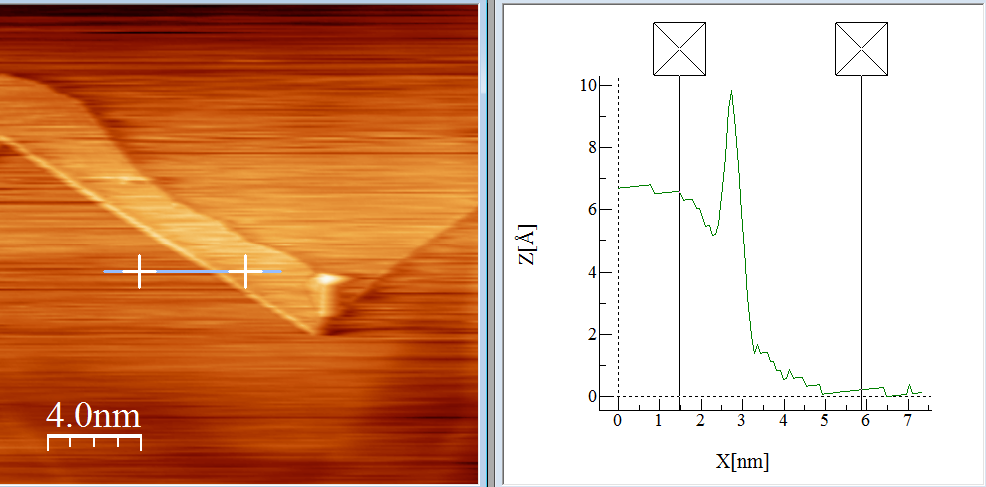
\includegraphics[scale = 0.2]{bild00.png}
	\centering
	\caption{Bild 0 Kante 0.637 nm}
	\label{b0}
\end{figure}

\begin{figure}[]
	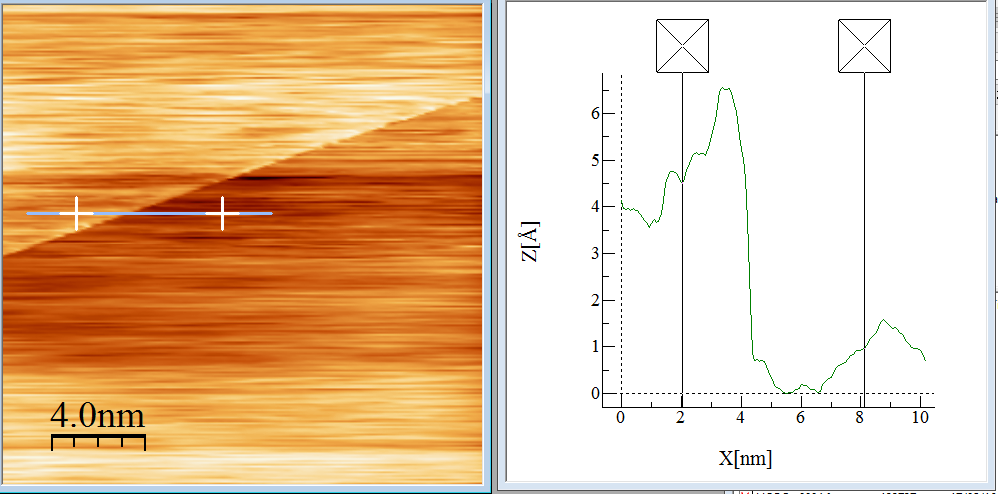
\includegraphics[scale = 0.2]{bild11.png}
	\centering
	\caption{Bild 11 Kante 0.353 nm}
	\label{b11}
\end{figure}
\begin{figure}[]
	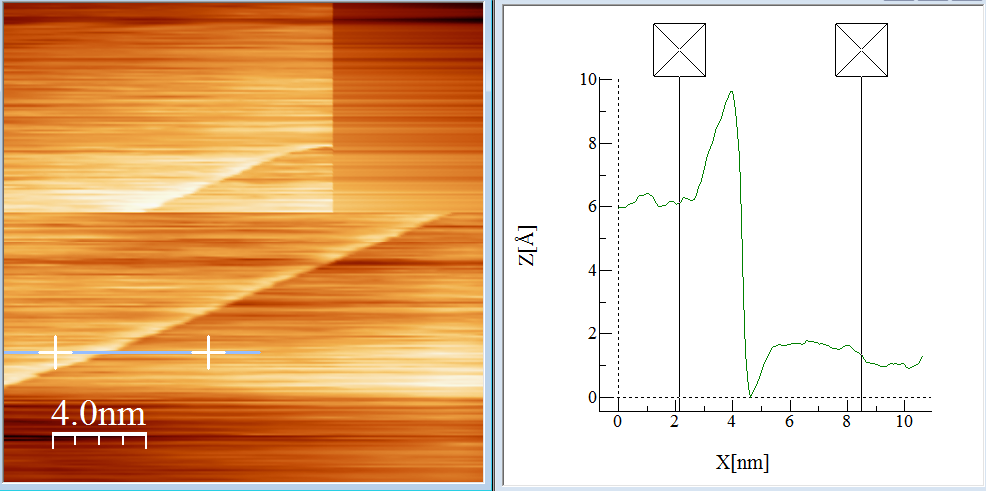
\includegraphics[scale = 0.2]{bild12.png}
	\centering
	\caption{Bild 12 Kante 0.447 nm}
	\label{b12}
\end{figure}

\begin{figure}[]
	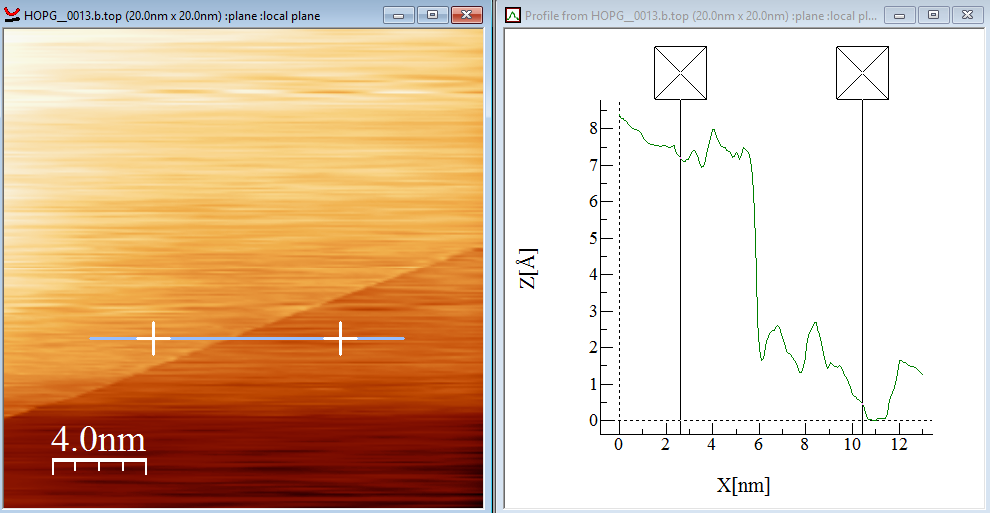
\includegraphics[scale = 0.2]{bild13.png}
	\centering
	\caption{Bild 13 Kante 0.677 nm}
	\label{b13}
\end{figure}

\begin{figure}[]
	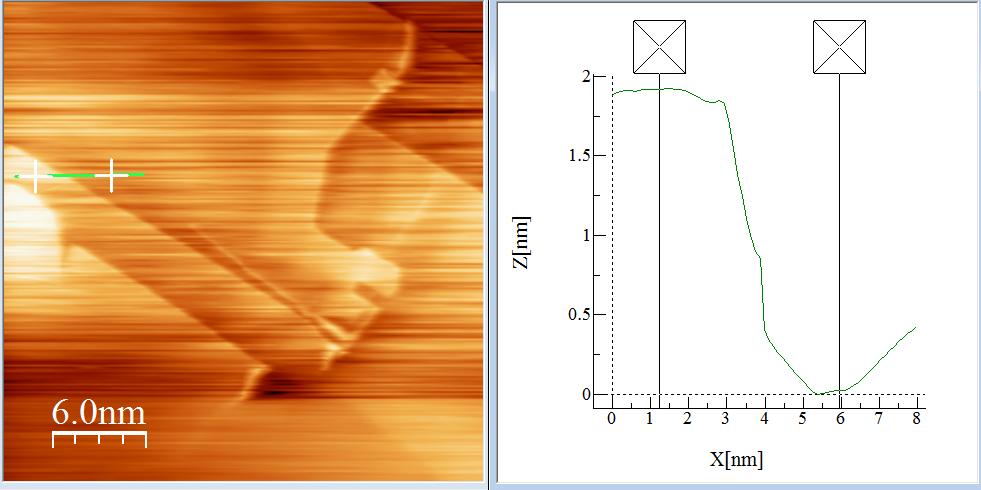
\includegraphics[scale = 0.2]{bild23.png}
	\centering
	\caption{Bild 23 Kante 1.896 nm}
	\label{b23}
\end{figure}
\begin{figure}[]
	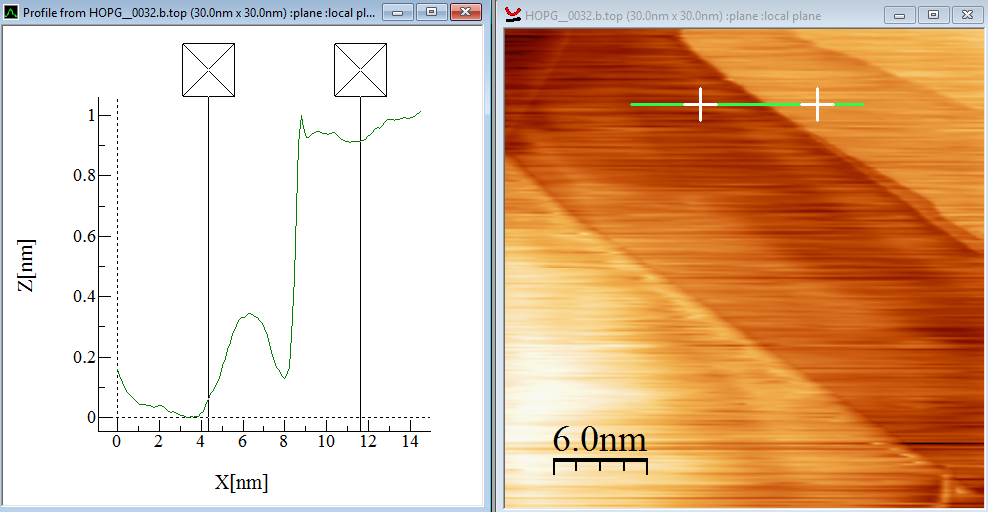
\includegraphics[scale = 0.2]{bild32.png}
	\centering
	\caption{Bild 32 Kante 0.853 nm}
	\label{b32}
\end{figure}

\begin{figure}[]
	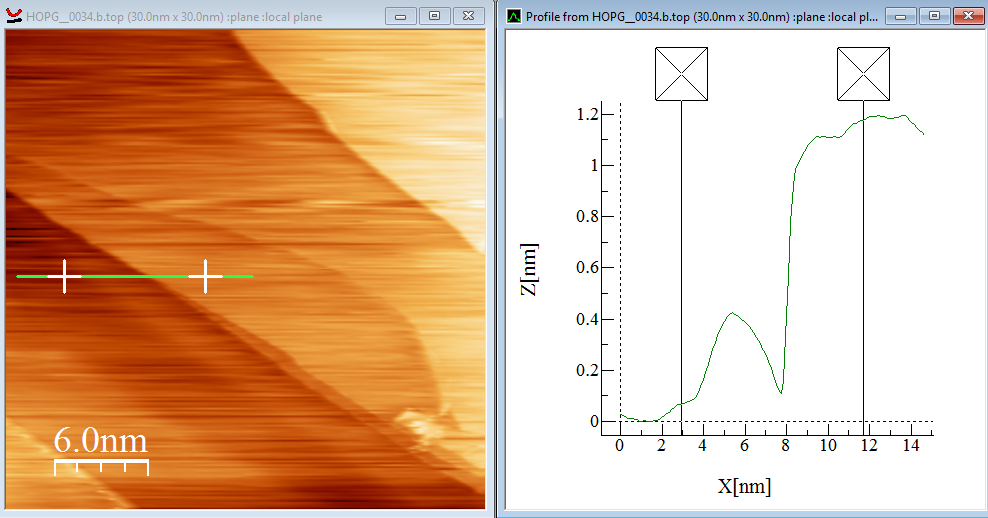
\includegraphics[scale = 0.2]{bild34.png}
	\centering
	\caption{Bild34 Kante 1.103 nm}
	\label{b34}
\end{figure}


\begin{figure}[]
	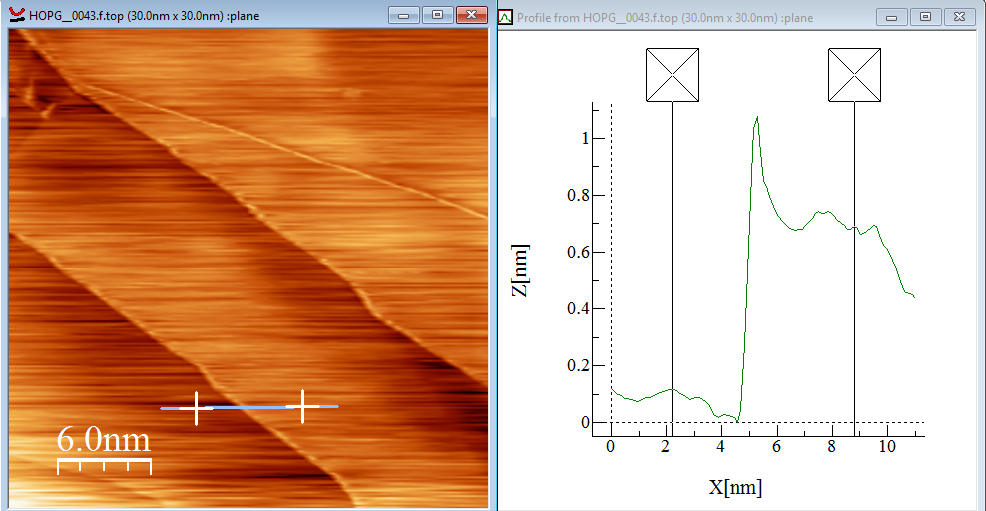
\includegraphics[scale = 0.2]{bild43.png}
	\centering
	\caption{Bild 43 Kante 0.572 nm}
	\label{b43}
\end{figure}

\begin{figure}[]
	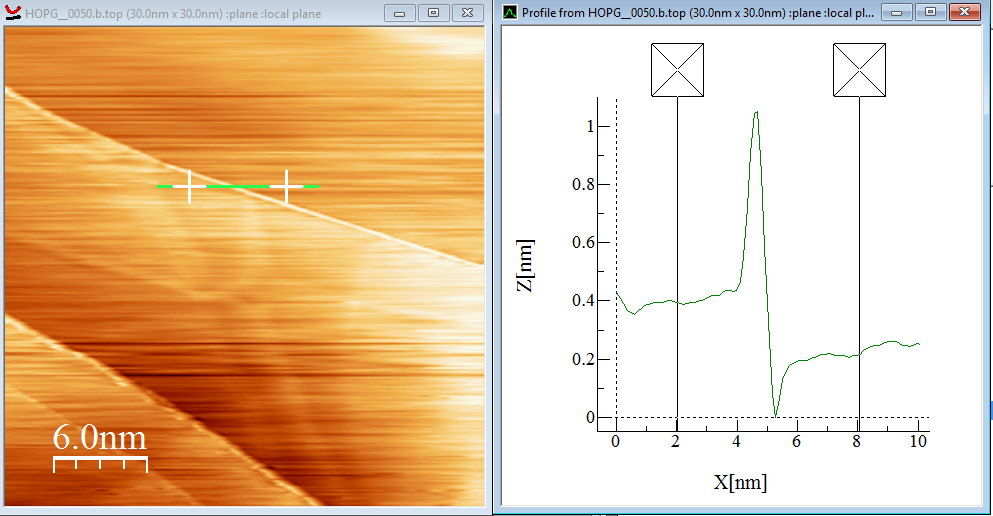
\includegraphics[scale = 0.2]{bild50.png}
	\centering
	\caption{Bild 50 Kante 0.179 nm}
	\label{b50}
\end{figure}

\begin{figure}[]
	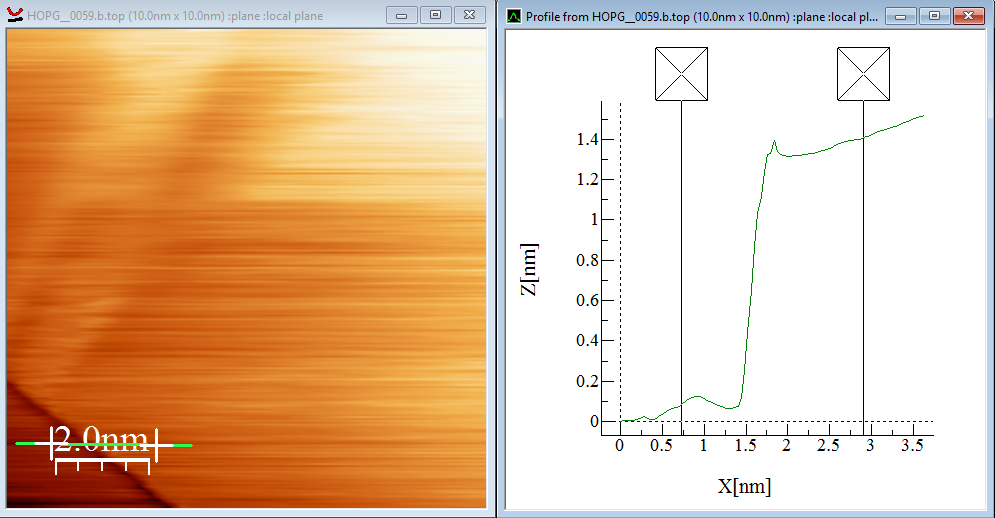
\includegraphics[scale = 0.2]{bild59.png}
	\centering
	\caption{Bild 59 Kante 1.302 nm}
	\label{b59}
\end{figure}

Nach dem wir alle Kanten vermessen haben, ordneten wir diese der Höhe nach. Die Höhen gingen von 0.179 nm bis 1.896 nm. Im folgenden haben wir die Höhen in einem Diagramm abgetragen und die theoretischen Kanten mit den roten Linien markiert.

\begin{figure}[]
	\includegraphics[scale = 0.5]{khglist.png}
	\centering
	\caption{Liste der ordeneten Kanten}
	\label{list}
\end{figure}

\begin{figure}[]
	\includegraphics[scale = 0.5]{khgdia.png}
	\centering
	\caption{Diagramm Höhe der Kanten sowie in Rot Theoretische Kantenhöhen}
	\label{list}
\end{figure}

In dem Diagramm zu den Höhen sehen wir eine Ansammlung von Kanten bei den N = 2 und 4 diese Kanten werden am besten durch unsere Messungen repräsentiert. Die anderen theoretischen Kanten werden nur bedingt durch unsere Messergebnisse wiedergespiegelt.
Beim Vergleichen der theoretischen Kanten mit dem Messergebissen muss drauf geachtet werden das die Kanten auch reale Kanten sind und keine Missinterpretation der Software. Die Form der Spitze ist auch entscheidend ob die Kanten "gut" erkennbar sind. Bei einigen Bildern waren die "Kanten" eher gebogen und dies kann bei einem Kristall nicht sein.

\section{Diskussion}

Das vermessen der Bilder ergab leider nur 16 Kanten. Diese Kanten sind nach der Höhe geordnet und im Diagramm 12 zu sehen. Wir konnten mit unseren Messergebnissen die theoretischen Kanten relativ gut darstellen. Vor allem den zweifachen und vierfachen Netzebenenabstand können unsere Messergebnisse rekonstruieren. Einige Messergebisse sind fast genau zwischen zwei Ebenen, dies könnte an der schlechte Wahl von Messpunkten am Bild liegen. Eine vorab Sondierung der Bilder wäre von Nöten gewesen mehr Kanten zu erfasst und die Ergebnisse klarer zu gestalten.

\end{document}